\chapter{Analysis}

In this chapter I will present the results of my analysis.\\
-I will present the results with the help of diagrams\\

-Describe the analysis that is done for each recording file we have:\\
-Show picture of a table with all the quantifiers as an axample and add the rest to the appendix\\
\begin{figure}
	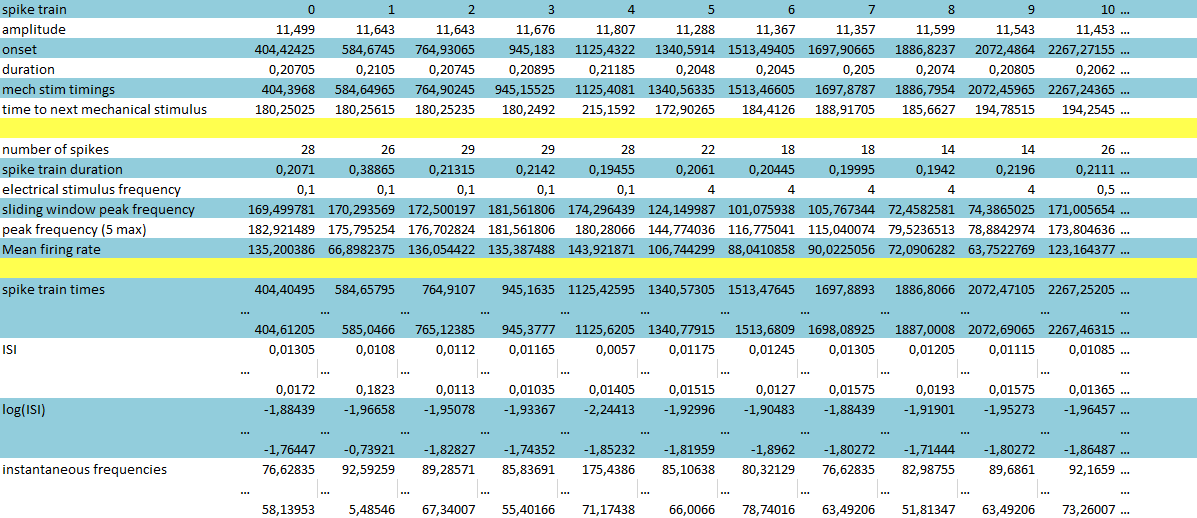
\includegraphics[width = \textwidth]{src/pic/sc_table}
	\caption{Sample picture of table after successful analysis }
	\label{fig:table_sc}
\end{figure}
-first batch contains information on the mechanical stimulus, second batch single number quantifiers about spike train, last batch lists of raw data and list quantifiers such as ISI\\
-with the help of this diagram describe the quantifiers and results that were computed\\


ausgewähltes in more detail:

-diagram of peak firing frequency, spike counts, train duration and electrical frequency\\
-shows the correlation between electrical frequency and the other quantifiers of single spike trains\\

-diagrams of Interspike Intervals(isi) and logarithm of isi\\
-should show that by taking the logarithm, the isi becomes more linear\\




\cleardoublepage
